\section[AMBIENTE DE ESTUDO]{AMBIENTE DE ESTUDO}

Como este trabalho trata de um projeto de desenvolvimento de software na área de análise de marcha, dois ambientes de trabalho distintos foram amplamente utilizados. São estes:

\begin{enumerate}
	\item Laboratório de Informática em Saúde (LIS) na Faculdade Gama (FGA) da Universidade de Brasília (UnB);
	\item Laboratório de Performance Humana (LPH) na Faculdade Ceilândia (FCE) da UnB.
\end{enumerate}

No LIS foram desempenhadas as tarefas relativas a engenharia de software e disponibilização do software.
Foram utilizadas estações de trabalho do tipo \emph{Power Mac} com sistema operacional \emph{MAC OS X} 10.10.3, sendo que uma foi preparada para funcionar como servidor de aplicação e roteador de rede. 
A estação preparada serve de hospedeira de duas máquinas virtuais (\emph{Virtual Machines} - VMs) rodando através do software \emph{Virtualbox} 4.3. 
Cada VM utiliza sistema operacional \emph{Debian Wheezy GNU/Linux}. 
Uma destas VMs foi configurada como roteador e \emph{firewall} e a outra como servidor de aplicações.  
Outra estação de trabalho \emph{Power Mac}, idêntica, e um \emph{notebook} rodando \emph{Ubuntu 14.04 GNU/Linux} foram utilizados como máquinas de desenvolvimento e simulação.
Um diagrama da rede criada no LIS é mostrado na Figura \ref{lis_rede}.

\begin{figure}[ht]
	\centering
	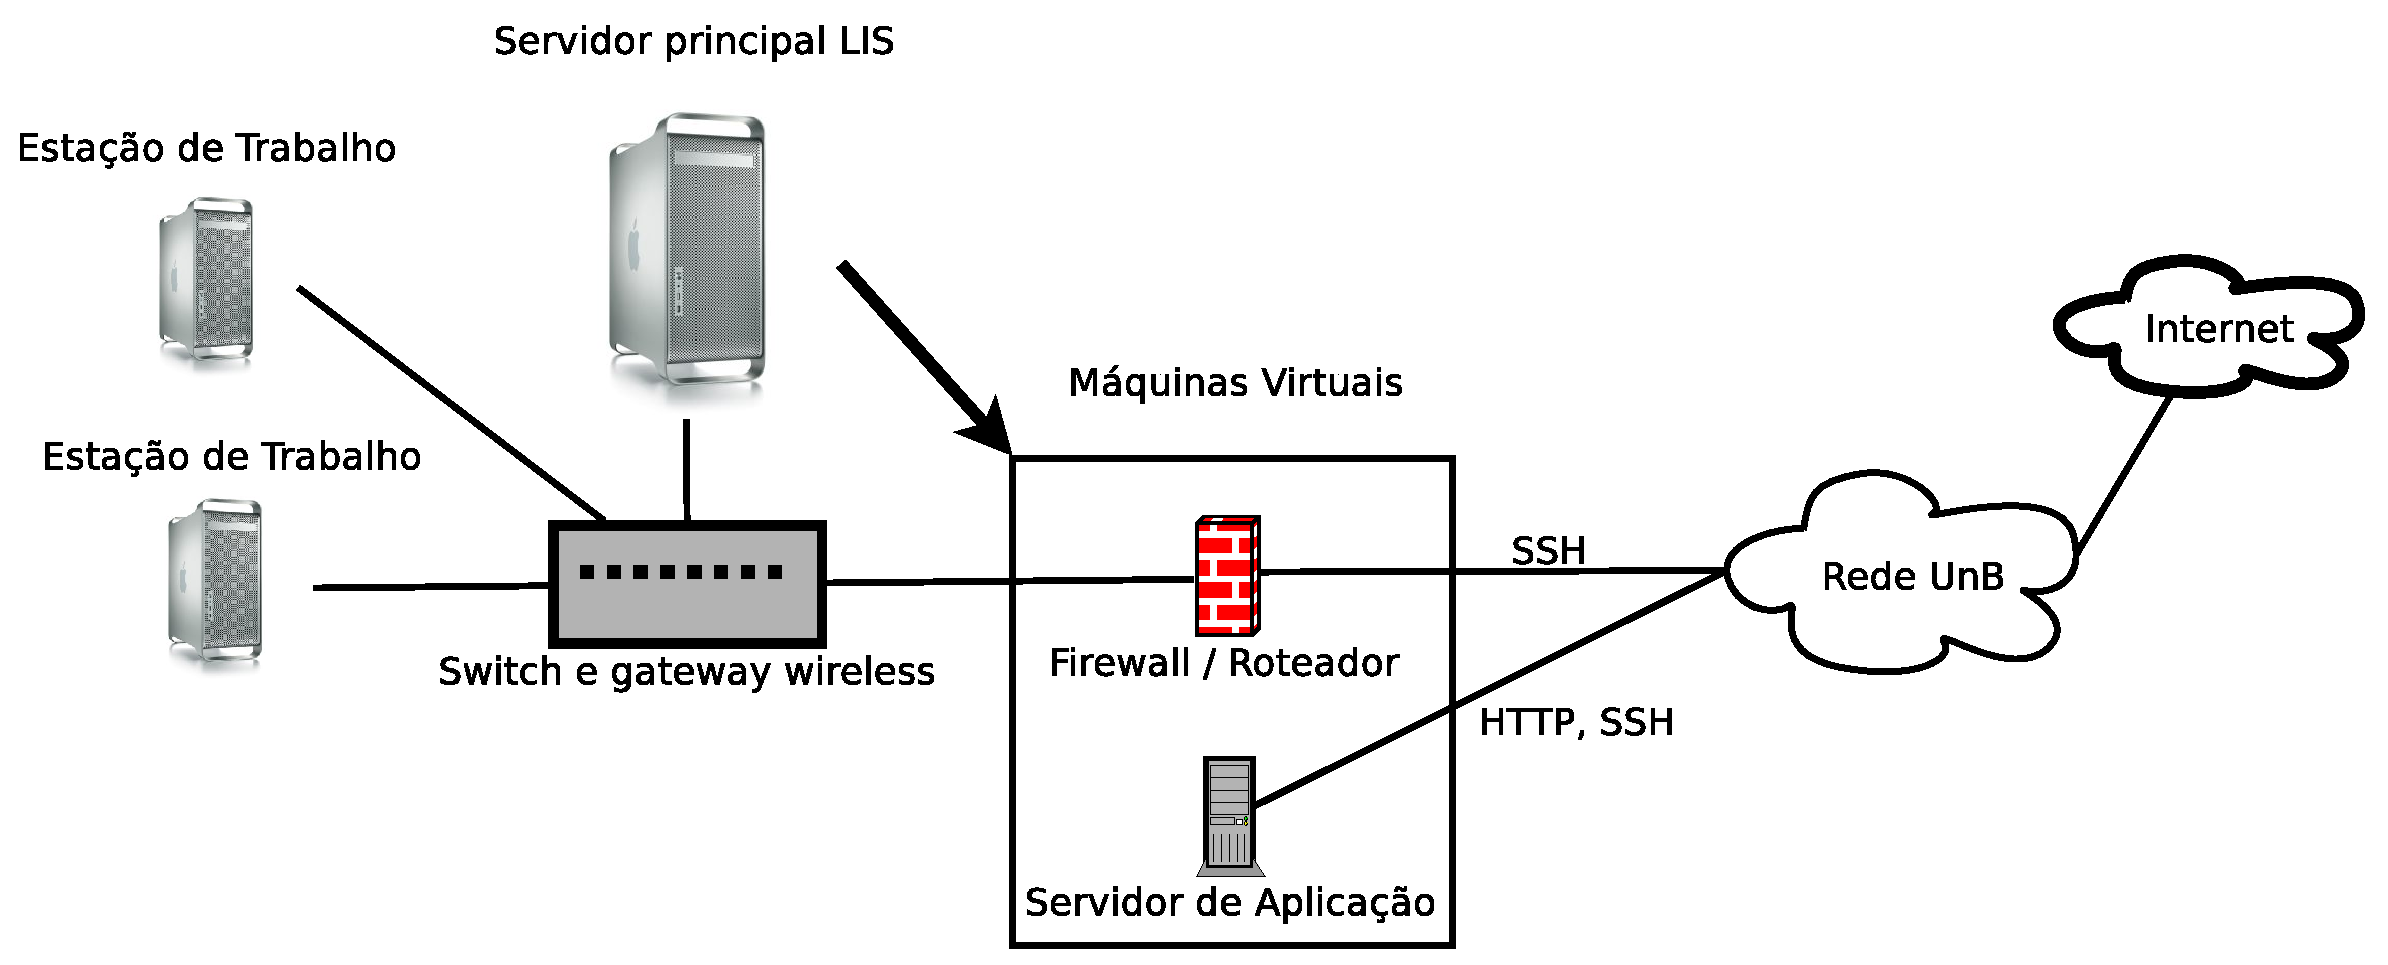
\includegraphics[width=15cm]{figuras/lis_rede.eps}
	\caption{Rede LIS.}
	\label{lis_rede}
\end{figure}

O LPH/FCE foi utilizado para captura de dados de marcha humana. 
Este laboratório está equipado para coletar dados de plataformas de força, eletromiógrafos e de marcadores posicionados no corpo do paciente através de câmeras de vídeo \emph{Oqus-MRI}, usando técnicas de (\emph{Motion Capture - MOCAP}), ver Figura \ref{oqus_mri}. 
Para este trabalho foi utilizado o software \emph{QTM 3.2} da \emph{Qualisys}, ver Figura \ref{visao_qtm}, que é responsável pela coleta de de dados \emph{MOCAP}. 

\begin{figure}[ht]
	\centering
	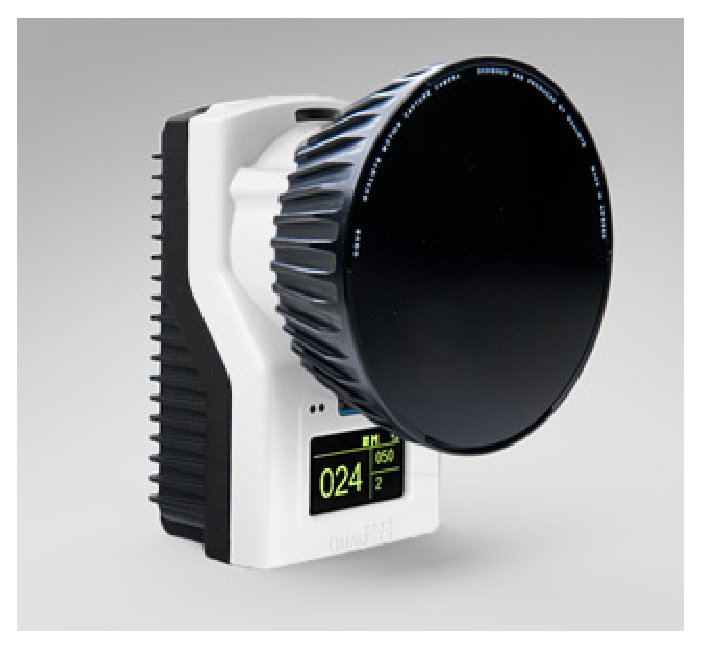
\includegraphics[width=7cm]{figuras/oqus-mri.eps}
	\caption{Camera Oqus MRI.}
	\label{oqus_mri}
	\footnotesize Fonte: \cite{Qualisys2013}.
\end{figure}


\begin{figure}[ht]
	\centering
	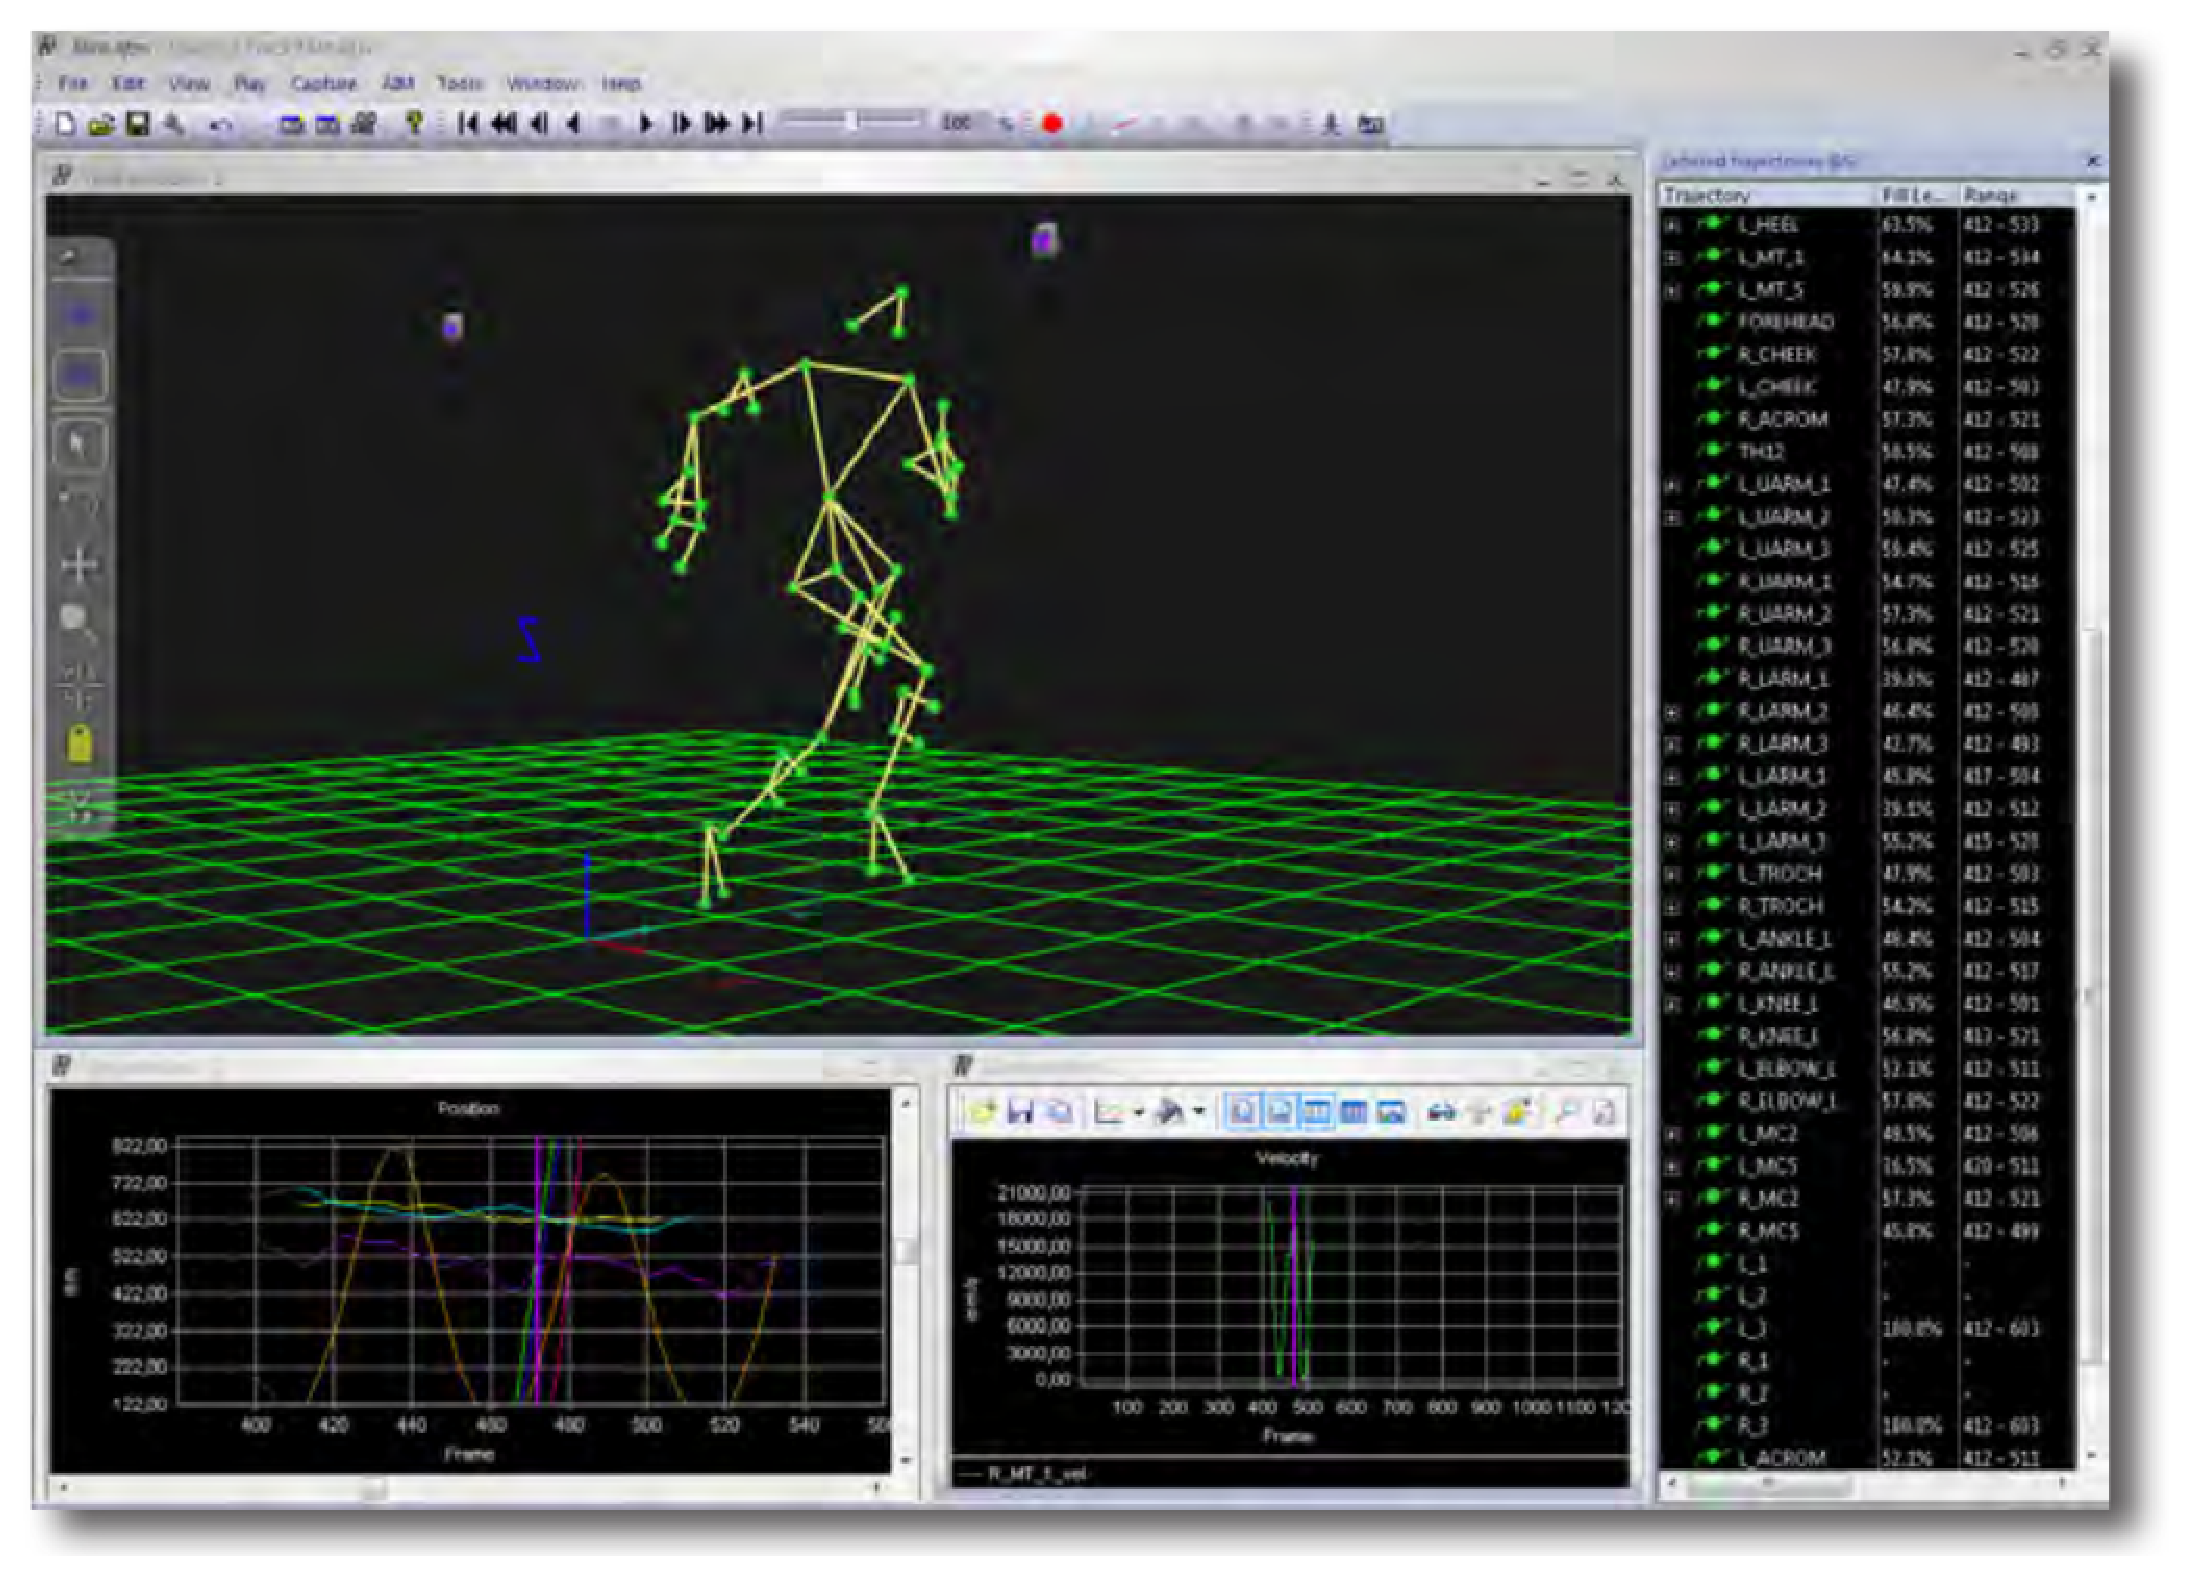
\includegraphics[width=10cm]{figuras/qtm.eps}
	\caption{Visão do QTM.}
	\label{visao_qtm}
	\footnotesize Fonte: \cite{Qualisys2010}.
\end{figure}

Os dados coletados para testar o sistema, são
dados cinemáticos, capturado através de motion capture,
utilizando-se de várias câmeras Qualisys Oqus MRI,
com marcadores passivos e pacote de software QTM 3.2
da Qualisys. Os dados foram convertidos para formato
adequado à linguagem Octave. Foram usados dados
capturados de um sujeito, no LPH da FCE/UnB.
Foi selecionado um sujeito sadio, do sexo masculino.
Este repetiu um ciclo de marcha de aproximadamente 5
segundos, por 5 vezes. Os dados trazem variáveis
espaciais, com respeito a posição dos marcadores. Os
marcadores estão distribuídos em 34 posições nas duas
pernas. Com estes
dados foram possíveis cálculos de angulações,
velocidades angulares e acelerações angulares. 
O projeto no qual ocorreu a coleta foi aprovado
pelo Comitê de Ética da Faculdade de Saúde da UnB,
processo N11911/12.
